\documentclass[11pt, a4paper]{article}

\usepackage{graphicx}
\usepackage[a4paper,top=3cm,bottom=2cm,left=2cm,right=2cm,marginparwidth=1.75cm]{geometry}
\usepackage[english]{babel}
\usepackage[utf8x]{inputenc}
\usepackage{subfig}
\usepackage{amsmath}
\usepackage{amssymb}

\graphicspath{ {./images} }
\newcommand*{\qed}{\hfill\ensuremath{\quad\square}}%
\newcommand*{\rad}{\ensuremath{\,\text{rad}}}
\newcommand*{\R}{\ensuremath{\mathbb{R}}}

\makeatletter
\renewcommand*\env@matrix[1][*\c@MaxMatrixCols c]{%
  \hskip -\arraycolsep
  \let\@ifnextchar\new@ifnextchar
  \array{#1}}
\makeatother

\newtheorem{theorem}{Theorem}

%------------------------------------------------
%Templates for images and figures
% \begin{figure}[h]
%   \centering
%   \subfloat[caption 1]{{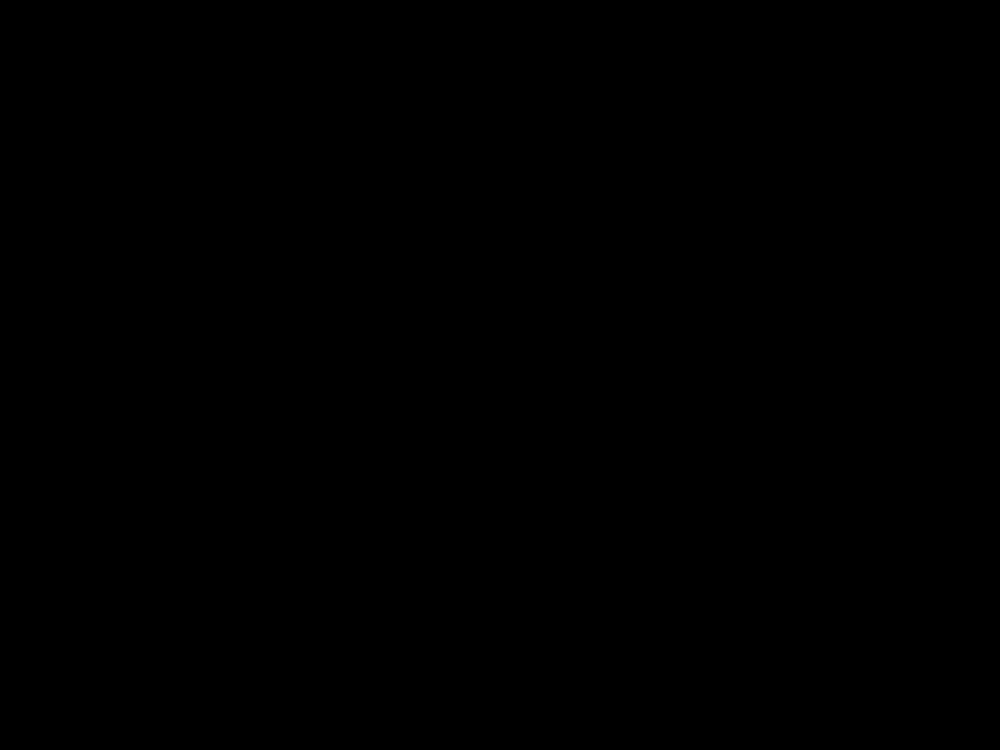
\includegraphics[width=30mm]{images/placeholder.png}}}%
%   \qquad
%   \subfloat[caption 2]{{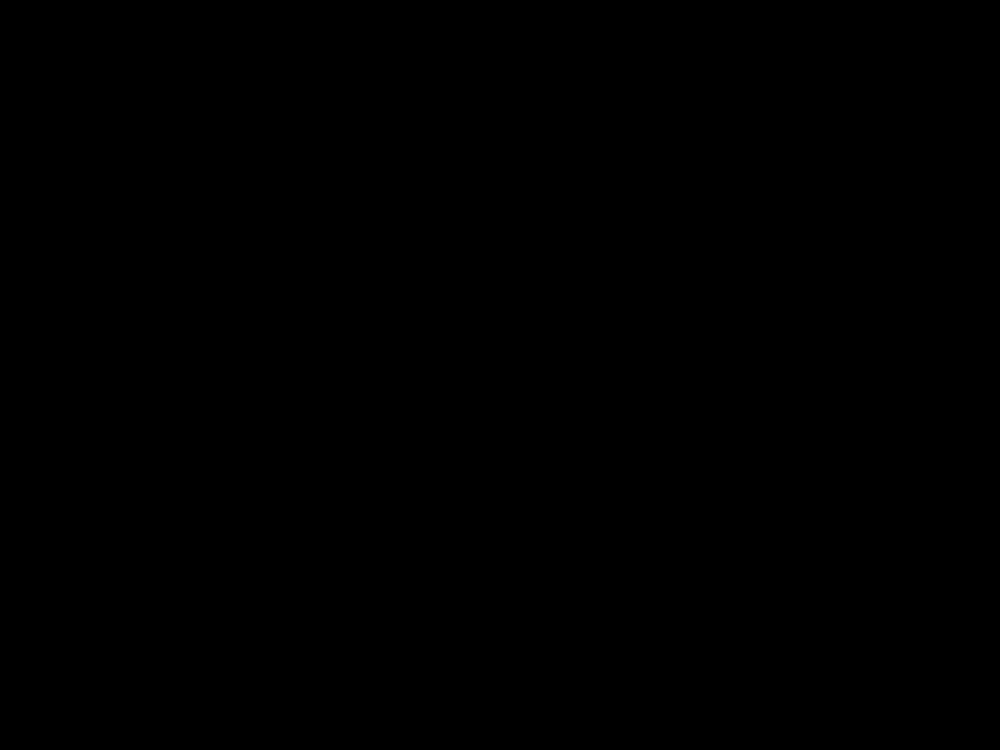
\includegraphics[width=30mm]{images/placeholder.png}}}%
%   \caption{Description}
% \end{figure}

% \begin{figure}[h]
%   \centerline{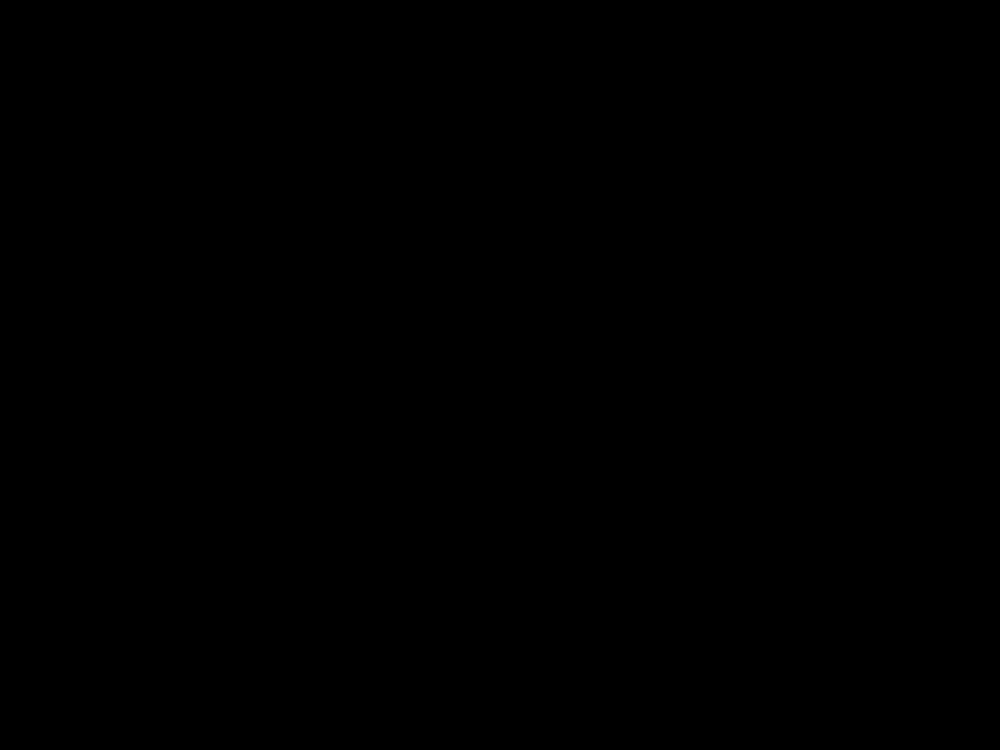
\includegraphics[width=50mm]{images/placeholder.png}}
%   \caption{Description}
% \end{figure}
%-----------------------------------------------

\begin{document}
\setcounter{equation}{0}
\setcounter{section}{6}
\section{Thermofluids Lecture 7: Control volume analysis (11/05/2020)}


\subsection{Recap: Table of different procceses}
\begin{table}[h]
  \caption{Equations for work and heat depending on the process.} %title of the table
  \centering % centering table
  \begin{tabular}{l|rr} % creating three columns
    \hline\hline %inserting double-line
  Process & $w_{12}$ & $q_{12}$\\ [0.5ex]
    \hline % inserts single-line
  Isochoric   & 0  & $c_v(T_2 - T_1)$\\ 
  Isobaric    & $p(v_2 - v_1)$ & $c_p(T_2 - T_1)$\\
  Isothermal  & $RT \ln \left(\frac{v_2}{v_1}\right)$ & $RT \ln \left(\frac{v_2}{v_1}\right)$\\
  Adiabatic   & $-c_v(T_2 - T_1)$  & 0\\
  \hline % inserts single-line
  \end{tabular}
  \label{tab:hresult}
\end{table}


\subsection{Open systems in thermodynamics}
An open system is any thermodynamic system where mass can cross the boundary of the system.. Examples of such systems are combustion engines and turbines. The law of conservation of mass still holds as it would for a closed system. However since mass is added from outside the system boundary we need to keep carefull track of what mass is added and what mass leaves the system. This leads to the follwing expression:
\begin{equation}
  \Delta m_{CV} = m_{in} - m_{out}
\end{equation}
This expression tells us that the net change in mass of the system is the mass entering the system minus the mass leaving the system. Contrast this with a closed system, where conservation of mass of the control volume tells us:
\begin{equation}
  m_1 = m_2
\end{equation}
Taking the time derrivative of expression (1) gives the following:
\begin{equation}
  \frac{dm_{CV}}{dt} = \dot{m_{in}} - \dot{m_{out}}
\end{equation}


\subsection{Energy balance of a flowing fluid}
Getting mass over the boundary of a system requires work. This work is usually called flow work. It is the amount of work required for pushing the fluid into the control volume at a constant velocity. We can say an imaginary piston pushes the fluid at constant speed into the control volume. The force required to do this is found to be $F = pA$ from the force balance, where $p$ is the fluid pressure and $A$ the cross-sectional area. We know mechanical work is $W = \int F\,ds$ and we also know our force is constant since both pressure and area stay contant. This leads to the following: $W_{12} = pA \cdot s$. When considering the pipe we can assert that $A\cdot s = V$ thus: $W_{12} = pV$ or written as an intensive property:
\begin{equation}
  w_{flow} = pv
\end{equation}
\newline
When we consider the energy equation of simple compressible flow in a unit mass basis we get:
\begin{equation}
  \Delta e = \Delta u + \Delta ke + \Delta pe = u + \frac{1}{2}V^2 + gz
\end{equation}
Where $V$ is the flow velocity and $z$ is the height relative to some randomly chosen datum. Note that this is for a closed system (i.e. mass does not enter the system from outside it's boundary). When considering the energy sum of a fluid entering or leaving a system boundary we need to account for the energy required for crossing the system boundary: flow energy. The total energy of a flowing fluid, denoted by the letter $\theta$ is then given by:
\begin{equation}
  \theta = pv + u + \Delta ke + \Delta pe
\end{equation}
$pv + u$ has earlier been defined as enthalpy, thus:
\begin{equation}
  \theta = h + \frac{1}{2}V^2 + gz
\end{equation}


\subsection{Energy transport by mass}
As we established earlier; The mass crossing the boundary of the system has energy. This means the mass going into and out of the system also carry energy into and out of the system. The total energy of a flowing fluid was earlier given in intensive form by $\theta$. We can multiply this value with mass to end up with the total amount of energy carried by the fluid:
\begin{gather}
  E_{mass} = m \theta = m \left( h + \frac{1}{2}V^2 + gz \right)\\
  \dot{E}_{mass} = \dot{m} \theta = \dot{m} \left( h + \frac{1}{2}V^2 + gz \right)
\end{gather}
When the kinetic and potential energy of a flowing fluid do not change (which is often the case depending on the system) we end up with:
\begin{gather}
  E_{mass} = mh\\
  \dot{E}_{mass} = \dot{m}h
\end{gather}


\subsection{Energy balance of an open system}
We now know how to describe the amount of mass transferred into and out of a system by mass transfer. When applying the first law to an open system we end up with:
\begin{equation}
  \Delta E = \Delta U + \Delta KE + \Delta PE = Q_{CV} - W_{CV} + \sum_{in} m_{in}\theta_{in} - \sum_{out} m_{out} \theta_{out} 
\end{equation}
Or when described in terms of rate of change:
\begin{equation}
  \frac{dE_{CV}}{dt} = \dot{Q}_{CV} - \dot{W}_{CV} + \sum_{in} \dot{m}_{in}\theta_{in} - \sum_{out} \dot{m}_{out} \theta_{out}
\end{equation}
When analysing a steady flow the change in energy over time is $0$. Written down as an equality: $\frac{dE_{CV}}{dt} = 0$. This allows us to rewrite equation (13) as:
\begin{equation}
  \dot{Q}_{in} + \dot{W}_{in} + \sum_{in} \dot{m}_{in} \theta_{in}  = \dot{Q}_{out} + \dot{W}_{out} + \sum_{out} \dot{m}_{out} \theta_{out}
\end{equation}

\end{document}
